\chapter{State Machines}\label{chap:state-machines}

%\section{State machines}\label{state_machine_sec}

State machines are an abstract model of step-by-step processes, and
accordingly, they come up in many areas of computer science.  You may
already have seen them in a digital logic course, a compiler course, or a
probability course.

\section{Basic definitions}

A state machine is really nothing more than a binary relation on a
set, except that the elements of the set are called ``states,'' the
relation is called the \term{transition relation}, and a pair $(p,q)$
in the graph of the transition relation is called a \term{transition}.
The transition from state $p$ to state $q$ will be written $p \movesto
q$.  The transition relation is also called the \term{state graph} of
the machine.  A state machine also comes equipped with a designated
\emph{start state}.

State machines used in digital logic and compilers usually have only a
finite number of states, but machines that model continuing computations
typically have an infinite number of states.  In many applications, the
states, and/or the transitions have labels indicating input or output
values, costs, capacities, or probabilities, but for our purposes,
unlabelled states and transitions are all we need.\footnote{We do name
states, as in Figure~\ref{fig:counter}, so we can talk about them, but the
names aren't part of the state machine.}

\begin{figure}[htbp]
\centering 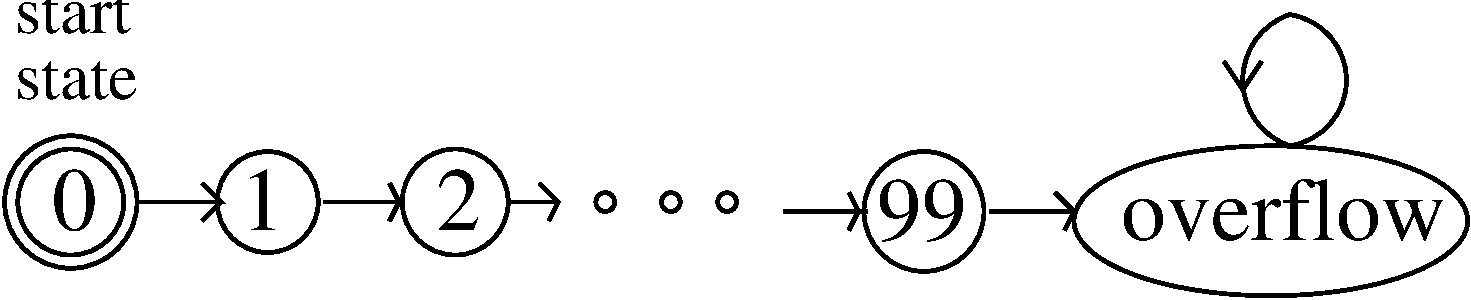
\includegraphics[height=1in]{counter}
%\centerline{\psfig{figure=counter.eps,height=1in}}
\caption{State transitions for the 99-bounded counter.}
\label{fig:counter}
\end{figure}

\begin{example}
A bounded counter, which counts from $0$ to $99$ and overflows at 100.
The transitions are pictured in Figure~\ref{fig:counter}, with start
state zero.  This machine isn't much use once it overflows, since it
has no way to get out of its overflow state.

\end{example}

\begin{example}
An unbounded counter is similar, but has an infinite state set.  This is
harder to draw \smiley\ .
\end{example}

\begin{example}
\textbf In the movie \textit{Die Hard 3: With a Vengeance}, the characters
played by Samuel L. Jackson and Bruce Willis have to disarm a bomb planted
by the diabolical Simon Gruber:

\textbox{
\begin{list}{}{\itemsep=0in \leftmargin=0.25in \rightmargin=0.25in}

\item[\textbf{Simon:}] On the fountain, there should be 2 jugs, do you
see them?  A 5-gallon and a 3-gallon.  Fill one of the jugs with
exactly 4 gallons of water and place it on the scale and the timer
will stop.  You must be precise; one ounce more or less will result in
detonation.  If you're still alive in 5 minutes, we'll speak.

\item[\textbf{Bruce:}] Wait, wait a second. I don't get it. Do you get it?

\item[\textbf{Samuel:}] No.

\item[\textbf{Bruce:}] Get the jugs. Obviously, we can't fill the 3-gallon jug
with 4 gallons of water.

\item[\textbf{Samuel:}] Obviously.

\item[\textbf{Bruce:}] All right. I know, here we go. We fill the 3-gallon jug
exactly to the top, right?

\item[\textbf{Samuel:}] Uh-huh.

\item[\textbf{Bruce:}] Okay, now we pour this 3 gallons into the 5-gallon jug,
giving us exactly 3 gallons in the 5-gallon jug, right?

\item[\textbf{Samuel:}] Right, then what?

\item[\textbf{Bruce:}] All right. We take the 3-gallon jug and fill it a third
of the way...

\item[\textbf{Samuel:}] No!  He said, ``Be precise.''  Exactly 4
gallons.

\item[\textbf{Bruce:}] Sh - -.  Every cop within 50 miles is running his a - - off
and I'm out here playing kids games in the park.

\item[\textbf{Samuel:}] Hey, you want to focus on the problem at hand?

\end{list}
}

Fortunately, they find a solution in the nick of time.  We'll let the
reader work out how.

The \emph{Die Hard} series is getting tired, so we propose a final
\emph{Die Hard Once and For All}.  Here Simon's brother returns to avenge
him, and he poses the same challenge, but with the 5 gallon jug replaced
by a 9 gallon one.

We can model jug-filling scenarios with a state machine.  In the scenario
with a 3 and a 5 gallon water jug, the states will be pairs, $(b,l)$ of
real numbers such that $0 \leq b \leq 5, 0 \leq l \leq 3$.  We let $b$ and
$l$ be arbitrary real numbers.  (We can prove that the values of $b$ and
$l$ will only be nonnegative integers, but we won't assume this.)  The
start state is $(0,0)$, since both jugs start empty.

Since the amount of water in the jug must be known exactly, we will only
consider moves in which a jug gets completely filled or completely
emptied.  There are several kinds of transitions:
\begin{enumerate}

\item  Fill the little jug: $(b,l) \movesto (b,3)$ for $l < 3$.

\item  Fill the big jug: $(b,l) \movesto (5,l)$ for $b<5$.

\item  Empty the little jug: $(b,l) \movesto (b,0)$ for $l>0$.

\item  Empty the big jug: $(b,l) \movesto (0,l)$ for $b>0$.

\item  Pour from the little jug into the big jug: for $l>0$,
\begin{equation*}
(b,l) \movesto
\begin{cases}
(b+l, 0) & \text{if $b + l \le 5$,}\\
(5, l - (5 - b)) & \text{otherwise.}
\end{cases}
\end{equation*}

\item Pour from big jug into little jug: for $b>0$,
\begin{equation*}
(b,l) \movesto
\begin{cases}
(0, b+l) & \text{if $b + l \le 3$,}\\
(b - (3 -l), 3) & \text{otherwise.}
\end{cases}
\end{equation*}
\end{enumerate}


Note that in contrast to the 99-counter state machine, there is more than
one possible transition out of states in the Die Hard machine.  Machines
like the 99-counter with at most one transition out of each state are
called \emph{deterministic}.  The Die Hard machine is
\emph{nondeterministic} because some states have transitions to several
different states.

\textbf{Quick exercise:} Which states of the Die Hard 3 machine have
direct transitions to exactly two states?

\end{example}

\section{Reachability and Preserved Invariants}

The Die Hard 3 machine models every possible way of pouring water among
the jugs according to the rules.  Die Hard properties that we want to
verify can now be expressed and proved using the state machine model.  For
example, Bruce's character will disarm the bomb if he can get to some
state of the form $(4, l)$.

A (possibly infinite) path through the state graph beginning at the
start state corresponds to a possible system behavior; such a path is
called an \term{execution} of the state machine.  A state is called
\term{reachable} if it appears in some execution.  The bomb in Die
Hard 3 gets disarmed successfully because the state (4,3) is
reachable.

\hyperdef{invariant}{properties}{A} useful approach in analyzing state
machine is to identify properties of states that are preserved by
transitions.  

\begin{definition}
  A \term{preserved invariant} of a state machine is a predicate, $P$, on
  states, such that whenever $P(q)$ is true of a state, $q$, and $q
  \movesto r$ for some state, $r$, then $P(r)$ holds.
\end{definition}

\textbox{\begin{center}
{\Large The Invariant Principle}
\end{center}

{\large
\noindent If a preserved invariant of a state machine is true for the
start state,\\
then it is true for all reachable states.}}

The Invariant Principle is nothing more than the Induction Principle
reformulated in a convenient form for state machines.  Showing that a
predicate is true in the start state is the base case of the induction,
and showing that a predicate is a preserved invariant is the inductive
step.\footnote{Preserved invariants are commonly just called
  ``invariants'' in the literature on program correctness, but we decided
  to throw in the extra adjective to avoid confusion with other
  definitions.  For example, another subject at MIT uses ``invariant'' to
  mean ``predicate true of all reachable states.''  Let's call this
  definition ``invariant-2.''  Now invariant-2 seems like a reasonable
  definition, since unreachable states by definition don't matter, and all
  we want to show is that a desired property is invariant-2.  But this
  confuses the \emph{objective} of demonstrating that a property is
  invariant-2 with the \emph{method} for showing that it is.  After all,
  if we already knew that a property was invariant-2, we'd have no need
  for an Invariant Principle to demonstrate it.}

\subsection{Die Hard Once and For All}

Now back to Die Hard Once and For All.  This time there is a 9 gallon jug
instead of the 5 gallon jug.  We can model this with a state machine whose
states and transitions are specified the same way as for the Die Hard 3
machine, with all occurrences of ``5'' replaced by ``9.''

Now reaching any state of the form $(4,l)$ is impossible.  We prove this
using the Invariant Principle.  Namely, we define the preserved invariant
predicate, $P(b,l)$, to be that $b$ and $l$ are nonnegative integer
multiples of 3.  So $P$ obviously holds for the state state $(0,0)$.

To prove that $P$ is a preserved invariant, we assume $P(b,l)$ holds for
some state $(b,l)$ and show that if $(b,l) \movesto (b',l')$, then
$P(b',l')$.  The proof divides into cases, according to which transition
rule is used.  For example, suppose the transition followed from the
``fill the little jug'' rule.  This means $(b,l) \movesto (b,3)$.  But
$P(b,l)$ implies that $b$ is an integer multiple of 3, and of course 3 is
an integer multiple of 3, so $P$ still holds for the new state $(b,3)$.
Another example is when the transition rule used is ``pour from big jug
into little jug'' for the subcase that $b + l > 3$.  Then state is $(b,l)
\movesto (b -( 3 -l), 3)$.  But since $b$ and $l$ are integer multiples of
3, so is $b -( 3 -l)$.  So in this case too, $P$ holds after the
transition.

We won't bother to crank out the remaining cases, which can all be checked
just as easily.  Now by the Invariant Principle, we conclude that every
reachable state satisifies $P$.  But since no state of the form $(4,l)$
satisifies $P$, we have proved rigorously that Bruce dies once and for
all!

By the way, notice that the state (1,0), which satisfies $\QNOT(P)$, has a
transition to (0,0), which satisfies $P$.  So it's wrong to assume that
the complement of a preserved invariant is also a preserved invariant.

\subsection{A Robot on a Grid}

There is a robot.  It walks around on a grid, and at every step it moves
diagonally in a way that changes its position by one unit up or down
\emph{and} one unit left or right.  The robot starts at position $(0, 0)$.
Can the robot reach position $(1, 0)$?

To get some intuition, we can simulate some robot moves.  For example,
starting at (0,0) the robot could move northeast to (1,1), then southeast
to (2,0), then southwest to (1,-1), then southwest again to (0,-2).

Let's model the problem as a state machine and then find a suitable
invariant.  A state will be a pair of integers corresponding to the
coordinates of the robot's position.  State $(i,j)$ has transitions to
four different states: $(i \pm 1, j \pm 1)$.

The problem is now to choose an appropriate preserved invariant, $P$, that
is true for the start state $(0,0)$ and false for $(1, 0)$.  The Invariant
Theorem then will imply that the robot can never reach $(1, 0)$.  A direct
attempt for a preserved invariant is the predicate $P(q)$ that $q \neq (1,
0)$.

Unfortunately, this is not going to work.  Consider the state $(2,1)$.
Clearly $P(2,1)$ holds because $(2,1) \neq (1, 0)$.  And of course
$P(1,0)$ does not hold.  But $(2,1) \movesto (1,0)$, so this choice of $P$
will not yield a preserved invariant.

We need a stronger predicate.  Looking at our example execution you might
be able to guess a proper one, namely, that the sum of the coordinates is
even!  If we can prove that this is a preserved invariant, then we have
proven that the robot never reaches $(1, 0)$ ---because the sum $1+0$ of
its coordinates is odd, while the sum $0+0$ of the coordinates of the
start state is even.

\begin{theorem}
The sum of the robot's coordinates is always even.
\end{theorem}

\begin{proof}
The proof uses the Invariant Principle.

Let $P(i, j)$ be the predicate that $i + j$ is even.

First, we must show that the predicate holds for the start state $(0,0)$.
Clearly, $P(0, 0)$ is true because $0 + 0$ is even.

Next, we must show that $P$ is a preserved invariant.  That is, we must
show that for each transition $(i, j) \movesto (i', j')$, if $i + j$ is
even, then $i' + j'$ is even.  But $i' = i \pm 1$ and $j' = j \pm 1$ by
definition of the transitions.  Therefore, $i' + j'$ is equal to $i + j$
or $i + j \pm 2$, all of which are even.
\end{proof}

\begin{corollary}
The robot cannot reach $(1, 0)$.
\end{corollary}

\textbox{
\begin{center}
{\Large Robert W. Floyd}
\end{center}

The Invariant Principle was formulated by Robert Floyd at Carnegie
Tech\footnote{The following year, Carnegie Tech was renamed
  Carnegie-Mellon Univ.} in 1967.  Floyd was already famous for work on
formal grammars which transformed the field of programming language
parsing; that was how he got to be a professor even though he never got a
Ph.D.  (He was admitted to a PhD program as a teenage prodigy, but flunked
out and never went back.)

In that same year, Albert R. Meyer was appointed Assistant Professor in
the Carnegie Tech Computer Science Department where he first met Floyd.
Floyd and Meyer were the only theoreticians in the department, and they
were both delighted to talk about their shared interests.  After just a
few conversations, Floyd's new junior colleague decided that Floyd was the
smartest person he had ever met.

Naturally, one of the first things Floyd wanted to tell Meyer about was
his new, as yet unpublished, Invariant Principle.  Floyd explained the
result to Meyer, and Meyer wondered (privately) how someone as brilliant
as Floyd could be excited by such a trivial observation.  Floyd had to
show Meyer a bunch of examples before Meyer understood Floyd's excitement
---not at the truth of the utterly obvious Invariant Principle, but rather
at the insight that such a simple theorem could be so widely and easily
applied in verifying programs.

Floyd left for Stanford the following year.  He won the Turing award
---the ``Nobel prize'' of computer science--- in the late 1970's, in
recognition both of his work on grammars and on the foundations of
program verification.  He remained at Stanford from 1968 until his
death in September, 2001.  You can learn more about Floyd's life and
work by reading the
\href{http://courses.csail.mit.edu/6.042/spring10/floyd-eulogy-by-knuth.pdf}{eulogy}
written by his closest colleague, Don Knuth.

 \iffalse
   \href{http://oldwww.acm.org/pubs/membernet/stories/floyd.pdf}
{\texttt{http://oldwww.acm.org/pubs/membernet/stories/floyd.pdf}}.
\fi
}

\section{Sequential algorithm examples}\label{seq_alg_subsec}

\subsection{Proving Correctness}

Robert Floyd, who pioneered modern approaches to program verification,
distinguished two aspects of state machine or process correctness:

\begin{enumerate}
\item The property that the final results, if any, of the process satisfy
system requirements.  This is called \emph{partial correctness}.

You might suppose that if a result was only partially correct, then it
might also be partially incorrect, but that's not what he meant.  The word
``partial'' comes from viewing a process that might not terminate as
computing a \emph{partial function}.  So partial correctness means that
when there is a result, it is correct, but the process might not always
produce a result, perhaps because it gets stuck in a loop.

\item The property that the process always finishes, or is guaranteed to
produce some legitimate final output.  This is called \emph{termination}.
\end{enumerate}

Partial correctness can commonly be proved using the Invariant Principle.
Termination can commonly be proved using the Well Ordering Principle.
We'll illustrate Floyd's ideas by verifying the Euclidean Greatest Common
Divisor (GCD) Algorithm.

\subsection{The Euclidean Algorithm}\label{euclid}

The \index{GCD algorithm}\term{Euclidean algorithm} is a
three-thousand-year-old procedure to compute the greatest common divisor,
$\gcd(a,b)$ of integers $a$ and $b$.  We can represent this algorithm as a
state machine.  A state will be a pair of integers $(x,y)$ which we can
think of as integer registers in a register program.  The state
transitions are defined by the rule
\[
(x,y) \movesto (y, \remainder(x,y))
\]
for $y \neq 0$.  The algorithm terminates when no further transition is
possible, namely when $y=0$.  The final answer is in $x$.

We want to prove:
\begin{enumerate}
\item Starting from the state with $x = a$ and $y = b>0$, if we ever finish,
then we have the right answer.  That is, at termination, $x = \gcd(a,b)$.
This is a \emph{partial correctness} claim.

\item We do actually finish.  This is a process \emph{termination} claim.

\end{enumerate}

\paragraph{Partial Correctness of GCD}

First let's prove that if GCD gives an answer, it is a correct answer.
Specifically, let $d \eqdef \gcd(a,b)$.  We want to prove that \emph{if}
the procedure finishes in a state $(x,y)$, then $x = d$.

\begin{proof}
Define the state predicate
\[
P(x,y) \eqdef\ \ [\gcd(x,y) = d \text{ and } (x > 0 \text{ or } y > 0)].
\]

$P$ holds for the start state $(a,b)$, by definition of $d$ and the
requirement that $b$ is positive.  Also, the preserved invariance of
$P$ follows immediately from
\begin{lemma}\label{gcdlem}
For all $m,n \in \naturals$ such that $n \neq 0$,
\begin{equation}
\gcd(m,n) = \gcd(n,\remainder(m,n)).
\end{equation}
\end{lemma}

Lemma~\ref{gcdlem} is easy to prove: let $q$ be the quotient and $r$
be the remainder of $m$ divided by $n$.  Then $m = qn +r$ by
definition.  So any factor of both $r$ and $n$ will be a factor of
$m$, and similarly any factor of both $m$ and $n$ will be a factor of
$r$.  So $r,n$ and $m,n$ have the same common factors and therefore
the same gcd.  Now by the Invariant Principle, $P$ holds for all
reachable states.

Since the only rule for termination is that $y=0$, it follows that if
$(x,y)$ is a terminal state, then $y=0$.  If this terminal state is
reachable, then the preserved invariant holds for $(x,y)$.  This implies
that $\gcd(x,0) = d$ and that $x>0$.  We conclude that $x = \gcd(x,0) =
d$.
\end{proof}

\paragraph{Termination of GCD}

Now we turn to the second property, that the procedure must terminate.  To
prove this, notice that $y$ gets strictly smaller after any one
transition.  That's because the value of $y$ after the transition is the
remainder of $x$ divided by $y$, and this remainder is smaller than $y$ by
definition.  But the value of $y$ is always a nonnegative integer, so by the
Well Ordering Principle, it reaches a minimum value among all its values
at reachable states.  But there can't be a transition from a state where
$y$ has its minimum value, because the transition would decrease $y$ still
further.  So the reachable state where $y$ has its minimum value is a
state at which no further step is possible, that is, at which the
procedure terminates.

Note that this argument does not prove that the minimum value of $y$ is
zero, only that the minimum value occurs at termination.  But we already
noted that the only rule for termination is that $y=0$, so it follows that
the minimum value of $y$ must indeed be zero.

\begin{editingnotes}
\subsubsection{The Extended Euclidean Algorithm}\label{ExtendedGCD}

An important fact about the $\gcd(a,b)$ is that it equals an integer
linear combination of $a$ and $b$, that is,
\begin{equation}\label{sa}
\gcd(a,b) = sa+ tb
\end{equation}
for some $s,t \in \integers$.  We'll see some nice proofs
of~\eqref{sa} later when we study Number Theory, but now we'll look
at an extension of the Euclidean Algorithm that efficiently, if
obscurely, produces the desired $s$ and $t$.  It is presented here
simply as another example of application of the Invariant Method
(plus, we'll need a procedure like this when we take up number theory
based cryptography in a couple of weeks).

\emph{Don't worry if you find this Extended Euclidean Algorithm hard to
  follow, and you can't imagine where it came from.  In fact, that's good,
  because this will illustrate an important point: given the right
  preserved invariant, you can verify programs you don't understand.}

In particular, given nonnegative integers $x$ and $y$, with $y>0$, we
claim the following procedure\footnote{This procedure is adapted from Aho,
  Hopcroft, and Ullman's text on algorithms.}  halts with registers
\texttt{S} and \texttt{T} containing integers $s$ and $t$
satisfying~\eqref{sa}.

Inputs: $a,b \in \naturals, b>0$.

Registers: \texttt{X,Y,S,T,U,V,Q}.

Extended Euclidean Algorithm:
\begin{center}
\begin{verbatim}
X := a; Y := b; S := 0; T := 1; U := 1; V := 0; 
loop:
if Y divides X, then halt
else
  Q := quotient(X,Y);
         ;;the following assignments in braces are SIMULTANEOUS
 {X := Y,
  Y := remainder(X,Y);
  U := S,
  V := T,
  S := U - Q * S,
  T := V - Q * T};
goto loop;
\end{verbatim}
\end{center}

Note that \texttt{X,Y} behave exactly as in the Euclidean GCD algorithm in
Section~\ref{euclid}, except that this extended procedure stops one step
sooner, ensuring that $\gcd(x,y)$ is in \texttt{Y} at the end.  So for all
inputs $x,y$, this procedure terminates for the same reason as the
Euclidean algorithm: the contents, $y$, of register \texttt{Y} is a
nonnegative integer-valued variable that strictly decreases each time
around the loop.

The following properties are preserved invariants that imply partial
correctness:
\begin{eqnarray}
\gcd(X,Y) &=& \gcd(a,b), \label{XY}\\
Sa+Tb &=& Y,\text{ and }\label{SaTb}\\
Ua+Vb &=& X. \label{uaVb}
\end{eqnarray}

To verify that these are preserved invariants, note that~\eqref{XY} is the
same one we observed for the Euclidean algorithm.  To check the other two
properties, let $x,y,s,t,u,v$ be the contents of registers
\texttt{X,Y,S,T,U,V} at the start of the loop and assume that all the
properties hold for these values.  We must prove that~\eqref{SaTb}
and~\eqref{uaVb} hold (we already know~\eqref{XY} does) for the new
contents $x',y',s',t',u',v'$ of these registers at the next time the loop
is started.

Now according to the procedure, $u'=s,v'=t,x'=y$, so~\eqref{uaVb} holds
for $u',v',x'$ because of~\eqref{SaTb} for $s,t,y$.  Also, 
\[
s'= u - qs,\quad t'= v - qt,\quad y' = x - qy
\]
where $q = \quotient(x,y)$,
so
\[
s'a+t'b = (u-qs)a + (v-qt)b =ua+vb - q(sa+tb) = x - qy = y',
\]
and therefore~\eqref{SaTb} holds for $s',t',y'$.

Also, it's easy to check that all three preserved invariants are true just
before the first time around the loop.  Namely, at the start:
\begin{align*}
X      =a, Y=b,S=0, T& =1 & \mbox{so}\\
Sa+Tb = 0a+1b=b& =Y & \mbox{confirming~\eqref{SaTb}.}
\end{align*}
Also,
\begin{align*}
U     & =1, V=0, & \mbox{so} \\
Ua+Vb & = 1a+0b=a =X & \mbox{confirming~\eqref{uaVb}.  }
\end{align*}
Now by the Invariant Principle, they are true at termination.  But at
termination, the contents, $Y$, of register \texttt{Y} divides the
contents, $X$, of register \texttt{X}, so preserved invariants~\eqref{XY}
and~\eqref{SaTb} imply
\[
\gcd(a,b) = \gcd(X,Y) = Y = Sa + Tb.
\]
So we have the gcd in register \texttt{Y} and the desired coefficients in
\texttt{S}, \texttt{T}.

Now we don't claim that this verification offers much insight.  In fact,
if you're not wondering how somebody came up with this concise program and
invariant, you:
\begin{itemize}

\item are blessed with an inspired intellect allowing you to see how this
  program and its invariant were devised,

\item have lost interest in the topic, or

\item haven't read this far.

\end{itemize}
If none of the above apply to you, we can offer some reassurance by
repeating that you're not expected to understand this program.
\end{editingnotes}

We've already observed that a preserved invariant is really just an
induction hypothesis.  As with induction, finding the right hypothesis
is usually the hard part.  We repeat:
\begin{quote}
  \textbf{Given the right preserved invariant, it can be easy to verify a
    program even if you don't understand it.}
\end{quote}
We expect that the Extended Euclidean Algorithm presented above
illustrates this point.

\section{Derived Variables}\label{derived_var_subsec}

The preceding termination proofs involved finding a nonnegative
integer-valued measure to assign to states.  We might call this measure
the ``size'' of the state.  We then showed that the size of a state
decreased with every state transition.  By the Well Ordering Principle,
the size can't decrease indefinitely, so when a minimum size state is
reached, there can't be any transitions possible: the process has
terminated.

\hyperdef{derived}{vars}{More} generally, the technique of assigning
values to states ---not necessarily nonnegative integers and not necessarily
decreasing under transitions--- is often useful in the analysis of
algorithms.  \emph{Potential functions} play a similar role in physics.
In the context of computational processes, such value assignments for
states are called \emph{derived variables}.

For example, for the Die Hard machines we could have introduced a derived
variable, $f: \text{states } \to \reals$, for the amount of water in both
buckets, by setting $f((a, b)) \eqdef a + b$.  Similarly, in the robot
problem, the position of the robot along the $x$-axis would be given by
the derived variable $x\text{-coord}$, where $x\text{-coord}((i, j))
\eqdef~i$.

We can formulate our general termination method as follows:

\begin{definition}
  Let $\prec$ be a strict partial order on a set, $A$.  A derived variable
  $f : \text{states } \to A$ is \emph{strictly decreasing} iff
\[
q \movesto q' \text{  implies  } f(q') \prec f(q).
\]
\end{definition}

We confirmed termination of the GCD and Extended GCD procedures by finding
derived variables, $y$ and \texttt{Y}, respectively, that were nonnegative
integer-valued and strictly decreasing.  We can summarize this approach to
proving termination as follows:
\begin{theorem}
\label{th:decr}
If $f$ is a strictly decreasing $\naturals$-valued derived variable of a
state machine, then the length of any execution starting at state $q$ is
at most $f(q)$.
\end{theorem}

Of course we could prove Theorem~\ref{th:decr} by induction on the value
of $f(q)$, but think about what it says: ``If you start counting down at
some nonnegative integer $f(q)$, then you can't count down more than
$f(q)$ times.''  Put this way, it's obvious.

\subsection{Weakly Decreasing Variables}

In addition being strictly decreasing, it will be useful to have derived
variables with some other, related properties.

\begin{definition}
Let $\preceq$ be a weak partial order on a set, $A$.  A derived variable
$f : Q \to A$ is \emph{weakly decreasing} iff
\[
q \movesto q' \text{  implies  } f(q') \preceq f(q).
\]

\emph{Strictly increasing} and \emph{weakly increasing} derived variables
are defined similarly.\footnote{Weakly increasing variables are often also
called \emph{nondecreasing}.  We will avoid this terminology to prevent
confusion between nondecreasing variables and variables with the much
weaker property of \emph{not} being a decreasing variable.}
\end{definition}

\begin{editingnotes}
\section*{Well-founded termination}
There are cases where it's easier to prove termination based on more
general partial orders than ``less-than'' on $\naturals$.  Termination is
guaranteed whenever there is a derived variable that strictly decreases with
respect to any well-founded partial order.

\textcolor{blue}{
We now define some other useful flavors of derived variables taking values
over partial ordered sets.  We'll use the notational convention that when
$\prec$ denotes a strict partial order on some set, then $\preceq$ is the
corresponding \emph{weak} partial order
\[
a\preceq a' \ \eqdef\quad a \prec a' \lor a = a'.
\]
}

\begin{definition}
Let $\prec$ be a strict partial order on a set, $A$.  A derived variable
$f : Q \to A$ is \emph{strictly decreasing} with respect to $\prec$ iff
\[
q \movesto q' \text{ implies } f(q') \prec f(q).
\]
Also, $f$ is \emph{weakly decreasing} iff
\[
q \movesto q' \text{  implies  } f(q') \preceq f(q).
\]
where $\preceq$ is the weak partial order corresponding to $\prec$,
namely,
\[
[a_1 \preceq a_2] \eqdef [(a_1 \prec a_2) \text{ or } (a_1=a_2)].
\]

\emph{Strictly increasing} and \emph{weakly increasing} derived variables
are defined similarly.\footnote{Weakly increasing variables are often also
called \emph{nondecreasing}.  We will avoid this terminology to prevent
confusion between nondecreasing variables and variables with the much
weaker property of \emph{not} being a decreasing variable.}
\end{definition}

\begin{theorem}\label{well-founded-decreasing}
  If there exists a derived variable for a state machine that is strictly
  decreasing with respect to some well-founded partial order, then every
  execution terminates.
\end{theorem}

Theorem~\ref{well-founded-decreasing} follows immediately from the
\href{http://courses.csail.mit.edu/6.042/spring08/ln3.pdf#infinite.decreasing}
{observation in Notes 3} that a well-founded partial order has no infinite
decreasing sequences.

Note that the existence of a nonnegative integer-valued \emph{weakly}
decreasing derived variable does not guarantee that every execution
terminates.  That's because an infinite execution could proceed through
states in which a weakly decreasing variable remained constant.

\subsubsection{A Southeast Jumping Robot}

\begin{staffnotes}Begin by defining the trivial ``pick how long'' game: P1 picks $n
\in \naturals$, the P2 and P1 alternate making forced moves.  The game
ends after $n$ forced moves; the last person to move wins.  So P1 strategy
is ``pick and even number.''  Insert here the discussion of ``terminates,
but no bound on number of steps...'' used below.

May also tell the ``guess a bigger number game''joke.
\end{staffnotes}

Here's a contrived but simple example of proving termination based on a
variable that is strictly decreasing over a well-founded order.  Let's
think about a robot positioned at an integer lattice-point in the
Northeast quadrant of the plane, that is, at $(x,y) \in \naturals^2$.

At every second when it is away from the origin, $(0,0)$, the robot must
make a move, which may be
\begin{itemize}

\item a unit distance West when it is not at the boundary of the Northeast
  quadrant (that is, $(x,y) \movesto (x-1,y)$ for $x>0$), or

\item a unit distance South combined with an arbitrary jump East (that is,
     $(x,y) \movesto (z,y-1)$ for $z\geq x$).

\end{itemize}
\begin{claim}\label{robotcl}
The robot will always get stuck at the origin.
\end{claim}

If we think of the robot as a nondeterministic state machine, then
Claim~\ref{robotcl} is a termination assertion.  The Claim may seem
obvious, but it really has a different character than termination based on
nonnegative integer-valued variables.  That's because, even knowing that
the robot is at position $(0,1)$, for example, there is no way to bound
the time it takes for the robot to get stuck.  It can delay getting stuck
for as many seconds as it wants by making its next move to a distant point
in the Far East.  This rules out proving termination using
Theorem~\ref{th:decr}.

So does Claim~\ref{robotcl} still seem obvious?

Well it is if you see the trick: if we reverse the coordinates, then every
robot move goes to a position that is smaller under lexicographic order.
More precisely, let $f:\naturals^2 \to \naturals^2$ be the derived variable
mapping a robot state ---its position $(x,y)$ ---to $(y,x) \in
\naturals^2$.  Now $(x,y)\movesto (x',y')$ is a legitimate robot move iff
$f((x',y')) \lex< f((x,y))$.  In particular, $f$ is a strictly
$\lex<$-decreasing derived variable, so
Theorem~\ref{well-founded-decreasing} proves that the robot always get
stuck as claimed.
\end{editingnotes}

\iffalse

We will prove that the robot always gets stuck at the origin by
generalizing the decreasing variable method, but with decreasing values
that are more general than nonnegative integers.  Namely, the traveling robot
can be modeled with a state machine with states of the form $((x,y),s,e)$
where
\begin{itemize}
\item $(x,y) \in \naturals^2$ is the robot's position,
\item $s$ is the number of moves South the robot took to get to this
position, and
\item $e \le 2s$ is the number of moves East the robot took to get to this
position. 
\end{itemize}

Now we define a derived variable $\vl:\text{States}\to \naturals^3$:
\[
\vl(((x,y),s,e)) \ \eqdef\quad (y,2s-e,x),
\]
and we order the values of states with the \emph{lexicographic} order,
$\lexle$, on $\naturals^3$:
\begin{equation}\label{lex3}
(k,l,m) \lexle (k',l',m') \ \eqdef\quad k < k' \text{ or } (k=k' \text{
and } l < l') \text{ or } (k=k' \text{ and } l = l' \text{ and } m \le m')
\end{equation}

Let's check that values are lexicographically decreasing.  Suppose the
robot is in state $((x,y),s,e)$.
\begin{itemize}
\item If the robot moves West it enters state $((x-1,y),s,e)$, and
\[
\vl(((x-1,y),s,e)) = (y,2s-e,x-1) \lex< (y,2s-e,x) = \vl(((x,y),s,e)),
\]
as required.


\item If the robot jumps East it enters a state $((z,y),s,e+1)$ for some
$z>x$.  Now
\[
\vl(((z,y),s,e+1)) = (y,2s-(e+1),z) = (y,2s-e-1,z),
\]
but since $2s-e-1 < 2s-e$, the rule~(\ref{lex3}) implies that
\[
\vl(((z,y),s,e+1)) = (y,2s-e-1,z)  \lex< (y,2s-e,x) = \vl(((x,y),s,e)),
\]
as required.

\item If the robot moves South it enters state $((x,y-1),s+1,e)$, and
\[
\vl(((x,y-1),s+1,e)) = (y-1,2(s+1)-e,x) \lex< (y,2s-e,x) = \vl(((x,y),s,e)),
\]
as required.

\end{itemize}

So indeed state-value is a decreasing variable under lexicographic order.
But since lexicographic order is well-founded, it is impossible for a
lexicographically-ordered value to be decreased an infinite number of
times.  That's just what we need to finish verifying Claim~\ref{robotcl}.
\fi

\begin{problems}
\homeworkproblems

\pinput{PS_filling_buckets_with_water}

\pinput{PS_linear_combination_game}

\pinput{PS_divide_using_3}

\pinput{PS_robot_on_2D_grid}

\pinput{PS_ant_on_grid}

\pinput{PS_card_shuffle_state_machine}

\pinput{PS_top_sort_for_closure_of_DAG}

\classproblems

\pinput{CP_fifteen_puzzle}

\pinput{CP_fast_exponentiation}

\pinput{CP_robot_invariant}

\pinput{CP_Zakim_bridge_state_machine}

\pinput{CP_98_heads_and_4_tails}

\pinput{CP_beaver_flu}

\end{problems}

\section{The Alternating Bit Protocol}

\begin{editingnotes}
Lynch Notes S07.H11-sm
\end{editingnotes}

The Alternating Bit Protocol is a well-known two-process communication
protocol that achieves reliable FIFO communication over unreliable
channels.  The unreliable channels may lose or duplicate messages, but
are assumed not to reorder them.  We'll use the
Invariant Method to verify that the Protocol

The Protocol allows a \textbf{Sender} process to send a sequence of
messages from a message alphabet, $M$, to a \textbf{Receiver}
process. It works as follows.

\textbf{Sender} repeatedly sends the rightmost message in its
\textbf{outgoing-queue} of messages, tagged with a \textbf{tagbit}
that is initially $1$.  When \textbf{Receiver} receives this tagged
message, it sets its \textbf{ackbit} to be the message tag $1$, and
adds the message to the lefthand end of its \textbf{received-msgs}
list.  Then as an acknowledgement, \textbf{Receiver} sends back
\textbf{ackbit} 1 repeatedly.  When \textbf{Sender} gets this
acknowledgement bit, it deletes the rightmost outgoing message in its
queue, sets its \textbf{tagbit} to 0, and begins sending the new
rightmost outgoing message, tagged with \textbf{tagbit}.

\textbf{Receiver}, having already accepted the message tagged with
\textbf{ackbit} $1$, ignores subsequent messages with tag $1$, and
waits until it sees the first message with tag $0$; it adds this
message to the lefthand side of its \textbf{received-msgs} list, sets
\textbf{ackbit} to 0 and acknowledges repeatedly with with
\textbf{ackbit} $0$.  \textbf{Sender} now waits till it gets
acknowledgement bit $0$, then goes on to send the next outgoing
message with tag $1$.  In this way, it alternates use of the tags $1$
and $0$ for successive messages.

We claim that this causes \textbf{Sender} to receive \emph{suffix}
original \textbf{outgoing-msgs} queue.  That is, at any stage in the
process when the the \textbf{outgoing-msgs}

(The fact that \textbf{Sender} actually outputs the entire outgoing
queuee is a \emph{liveness} claim ---liveness properties are a
generalization of termination properties.  We'll ignore this issue for
now.)

We formalize the description above as a state whose states consist of:
\begin{tabbing}
XXX\=XXX\= \kill \> $\text{\textbf{outgoing-msgs}}$, a finite sequence of $M$,
whose initial value is called \textbf{all-msgs}\\ \> $\text{\textbf{tagbit}} \in
\set{0, 1}$, initially $1$ \\ \\ \> $\text{\textbf{received-msgs}}$, a finite
sequence of $M$, initially empty\\ \> $\text{\textbf{ackbit}}( \in \set{0, 1}$,
initially $0$ \\ \\ \> $\text{\textbf{msg-channel}}$, a finite sequence of $M
\times \set{0, 1}$, initially empty, \\ \> $\text{\textbf{ack-channel}}$, a
finite sequence of $\set{0, 1}$, initially empty
\end{tabbing}

The transitions are:
\begin{enumerate}
\item[\textbf{SEND:}]

\begin{enumerate}
\item
\prcef{$\text{\textbf{send-msg}}(m,b)$}
{% Pre: 
   $m = \text{\textbf{rightend}}(\text{\textbf{outgoing-msgs}}) \QAND
   b = \text{\textbf{tagbit}}$}
{% Eff: 
   add $(m,b)$ to the lefthand end of $\text{\textbf{msg-channel}}$,
   any number $\geq 0$ of times}

\item
\prcef{$\text{\textbf{send-ack}}(b)$}
{% Pre: 
   $b = \text{\textbf{ackbit}}$}
{% Eff: 
   add $b$ to the righthand end of $\text{\textbf{ack-channel}}$,
   any number $\geq 0$ of times}
\end{enumerate}

\item[\textbf{RECEIVE:}]

\begin{enumerate}
\item
\prcef{$\text{\textbf{receive-msg}}(m,b)$}
 {% Pre: 
   $(m,b) = \text{\textbf{rightend}}(\text{\textbf{msg-channel}})$}
{% Eff: 
   remove $\text{\textbf{rightend}}$ of $\text{\textbf{msg-channel}}$;\\
   if $b \neq \text{\textbf{ackbit}}$, then
   [add $m$ to the lefthand end of $\text{\textbf{receive-msgs}}$;
   $\text{\textbf{ackbit}} := b$.]}

\item \prcef{$\text{\textbf{receive-ack}}(b)$}
{% Pre: 
   $b = \text{\textbf{leftend}}(\text{\textbf{ack-channel}}()$}
{% Eff: 
   remove $\text{\textbf{leftend}}$ of $\text{\textbf{ack-channel}}$.\\
   if $b = \text{\textbf{tagbit}}$, then
   [remove $\text{\textbf{rightend}}$ of $\text{\textbf{outgoing-msgs}}$ (if nonempty);
   $\text{\textbf{tagbit}} := \bar{\text{\textbf{tagbit}}}$]}
\end{enumerate}

\end{enumerate}

Our goal is to show that when $\text{\textbf{tagbit}} \neq
\text{\textbf{ackbit}}$, then\\
\begin{equation}\label{all-msgs-preserved}
\text{\textbf{outgoing-queue}}\cdot \text{\textbf{received-msgs}} =
\text{\textbf{all-msgs}}.
\end{equation}

This requires three auxiliary invariants.
For the first of these, we need a definition.

Let $\text{\textbf{tag-sequence}}$ be the sequence consisting of bits in
$\text{\textbf{ack-channel}}$, in right-to-left order, 
followed by $\text{\textbf{tagbit}}$, 
followed by the tag components of the elements of
$\text{\textbf{msg-channel}}$, in left-to-right order, 
followed by $\text{\textbf{ackbit}}$. 

{\bf Property 2:}
$\text{\textbf{tag-sequence}}$ consists of one of the following:
\begin{enumerate}
\item
All $0$'s.
\item
All $1$'s. 
\item
A positive number of $0$'s followed by a positive number of $1$'s.
\item
A positive number of $1$'s followed by a positive number of $0$'s.
\end{enumerate}
What is being ruled out by these four cases is the situation where
the sequence contains more than one switch of tag value. 

The fact that Property 2 is an invariant can be proved easily by
induction.  We also need: 

{\bf Property 3:}
If $(m,\text{\textbf{tag}})$ is in $\text{\textbf{msg-channel}}$ then $m =
\text{\textbf{rightend}}(\text{\textbf{outgoing-queue}})$. \\

\begin{proof}
(That Property 3 is an invariant)

By induction, using Property 2. 

Base: Obvious, since no message is in the channel initially. 

Inductive step: It is easy to see that the property is preserved by
$\text{\textbf{send}}_{m,b}$, which adds new messages to $\text{\textbf{channel}}_{1,2}$.
The only other case that could cause a problem is
$\text{\textbf{receive}}(b)_{2,1}$,
which could cause $\text{\textbf{tag}}_1$ to change when there is another message
already in $\text{\textbf{channel}}_{1,2}$ with the same tag. 
But this can't happen, by Property 2 applied before the step -- since
the incoming tag $g$ must be equal to $\text{\textbf{tag}}_1$ in this case,
all the tags in $\text{\textbf{tag-sequence}}$ must be the same.
\end{proof}

Finally, we need that the following counterpart
to~\eqref{all-msgs-preserved}: when $\text{\textbf{tagbit}} =
\text{\textbf{ackbit}}$, then
\begin{equation}\label{all-msgs-preserved2}
\text{\textbf{lefttail}(\textbf{outgoing-queue})}\cdot \text{\textbf{received-msgs}} =
\text{\textbf{all-msgs}},
\end{equation}
where $\text{\textbf{lefttail}}(\textbf{outgoing-queue})$ all but the
rightmost message, if any, in \textbf{outgoing-queue}.

Property 4, part 2, easily implies the goal Property 1.
It also implies that $\text{\textbf{work-buf}}_2$ is always nonempty when 
$\text{\textbf{receive}}(b)_{2,1}$ occurs with equal tags; therefore, the
parenthetical check in the code always works out to be true.

\begin{proof}
(That Property 4 is an invariant)

By induction. 
Base: In an initial state, the tags are unequal, 
$\text{\textbf{work-buf}}_1 = \text{\textbf{buf}}_1$ and $\text{\textbf{buf}}_2$ is empty.  This
suffices to show part 1.  part 2 is vacuous.

Inductive step:
When a $\text{\textbf{send}}$ occurs, the tags and buffers are unchanged, so the
truth of the invariants must be preserved. 
It remains to consider $\text{\textbf{receive}}$ events.

$\text{\textbf{receive}}(m,b)_{1,2}$:

If $b = \text{\textbf{tag}}_2$, nothing happens, so the invariants are
preserved.  So suppose that $b \neq \text{\textbf{tag}}_2$.  Then
Property 2 implies that $b = \text{\textbf{tag}}_1$, and then Property
3 implies that $m$ is the first message on
$\text{\textbf{work-buf}}_1$.  The effect of the transition is to
change $\text{\textbf{tag}}_2$ to make it equal to
$\text{\textbf{tag}}_1$, and to replicate the first element of
$\text{\textbf{work-buf}}22_1$ at the end of $\text{\textbf{buf}}_2$.

The inductive hypothesis implies that, before the step,
$\text{\textbf{buf}}_2 \cdot \text{\textbf{work-buf}}_1 =
\text{\textbf{buf}}_1$.  The changes caused by the step imply that,
after the step, $\text{\textbf{tag}}_1 = \text{\textbf{tag}}_2$,
$\text{\textbf{work-buf}}_1$ and $\text{\textbf{buf}}_2$ are nonempty,
$\text{\textbf{head}}(\text{\textbf{work-buf}}_1) =
\text{\textbf{last}}(\text{\textbf{buf}}_2)$, and
$\text{\textbf{buf}}_2 \cdot
\text{\textbf{tail}}(\text{\textbf{work-buf}}_1) =
\text{\textbf{buf}}_1$.  This is as needed.

$\text{\textbf{receive}}(b)_{2,1}$:

The argument is similar to the one for
$\text{\textbf{receive}}(m,b)_{1,2}$.  If $b \neq
\text{\textbf{tag}}_1$, nothing happens so the invariants are
preserved.  So suppose that $b = \text{\textbf{tag}}_1$.  Then
Property 2 implies that $b = \text{\textbf{tag}}_2$, and the step
changes $\text{\textbf{tag}}_1$ to make it unequal to
$\text{\textbf{tag}}44_2$.  The step also removes the first element of
$\text{\textbf{work-buf}}_1$.  The inductive hypothesis implies that,
before the step, $\text{\textbf{work-buf}}_1$ and
$\text{\textbf{buf}}_2$ are nonempty,
$\text{\textbf{head}}(\text{\textbf{work-buf}}_1) =
\text{\textbf{last}}(\text{\textbf{buf}}_2)$, and
$\text{\textbf{buf}}_2 \cdot
\text{\textbf{tail}}(\text{\textbf{work-buf}}_1) =
\text{\textbf{buf}}_1$.  The changes caused by the step imply that,
after the step, $\text{\textbf{tag}}_1 \neq \text{\textbf{tag}}_2$ and
$\text{\textbf{buf}}_2 \cdot \text{\textbf{work-buf}}_1 =
\text{\textbf{buf}}_1$.  This is as needed.
\end{proof}

\section{Reasoning About \textbf{While} Programs}\label{while_chap}

Real programs and programming languages are often huge and complicated,
making them hard to model and even harder to reason about.  Still, making
programs ``reasonable'' is a crucial aspect of software engineering.  In
this section we'll illustrate what it means to have a clean mathematical
model of a simple programming language and reasoning principles that go
with it ---if only real programming languages allowed for such simple,
accurate modeling.

\subsection{\textbf{While} Programs}

The programs we'll study are called ``\term{\while\ programs}.''  We
can define them as a recursive data type:
\begin{definition}\label{whiledef} \mbox{}

\textbf{base cases:}
\begin{itemize}

\item $x \assigned e$ is a \while\ program, called an \term{assignment
    statement}, where $x$ is a variable and $e$ is an expression.

\item \term{$\halt$} is a \while\ program.

\end{itemize}

\textbf{constructor cases:}
If $C$ and $D$ are \while\ programs, and $T$ is a test, then the following are also
\while\ programs:
\begin{itemize}

\item $\seqcomm{C}{D}$
---called the \term{sequencing} of $C$ and $D$,

\item $\condcomm{T}{C}{D}$ ---called a \term{conditional} with
  \term{test}, $T$, and \term{branches}, $C$ and $D$,

\item $\wloop{T}{C}$
---called a \term{while loop} with \term{test}, $T$, and \term{body}, $C$.

\end{itemize}
\end{definition}

For simplicity we'll stick to \while\ programs operating on integers.  So by
expressions we'll mean any of the familiar integer valued
expressions involving integer constants and operations such as addition,
multiplication, exponentiation, quotient or remainder.  As \term{tests},
we'll allow propositional formulas built from basic formulas of the form
$e \leq f$ where $e$ and $f$ are expressions.  For example, here is the
Euclidean algorithm for $\gcd(a,b)$ expressed as a \while\ program.
\begin{tabbing}
XXX\=XXX\=XXX\=XXX\kill
$\mathtt{x} \assigned a$\textbf{;} \\
$\mathtt{y} \assigned b$\textbf{;} \\
\while\ $\mathtt{y} \neq 0$ \docomm\\
   \> $\mathtt{t} \assigned \mathtt{y}$\textbf{;}\\
   \> $\mathtt{y} \assigned \rem{\mathtt{x}}{\mathtt{y}}$\textbf{;}\\
   \> $\mathtt{x} \assigned \mathtt{t}$
\odcomm\\
\end{tabbing}

\subsection{The \textbf{While}  Program State Machine}

A \while\ program acts as a pure command: it is run solely for its
side effects on stored data and it doesn't return a value.  The data
consists of integers stored as the values of variables, namely
environments:
\begin{definition}
An \term{environment} is a total function from variables to integers.
Let $\Env$ be set of all environments.
\end{definition}
So if $\rho$ is an environment and $x$ is a variable, then $\rho(x)$ is an
integer.  More generally, the environment determines the integer value of
each expression, $e$, and the truth value of each test, $T$.  We can think
of an expression, $e$ as defining a function $\mean{e}:\Env \to
\integers$, and refer to this function, $\mean{e}$ as the \term{meaning}
of $e$, and likewise for tests.

It's standard in programming language theory to write $\mean{e}\rho$
as shorthand for $\mean{e}(\rho)$, that is, applying
the \emph{meaning}, $\mean{e}$, of $e$ to $\rho$.  For example, if
$\rho(\mathtt{x}) =4$, and $\rho(\mathtt{y}) =-2$, then
\begin{equation}\label{x2y311}
\mean{\mathtt{x^2+y -3}}\rho = \rho(\mathtt{x})^2 + \rho(y) -3 = 11.
\end{equation}

\iffalse
(A variable is a special case of an expression, so $\mean{x}\rho \eqdef \rho(x)$.)
\fi

Executing a program causes a succession of changes to the
environment\footnote{More sophisticated programming models distinguish
the environment from a \term{store} which is affected by commands, but
this distinction is unnecessary for our purposes.}  which may continue
until the program halts.  Actually the only command which immediately
alters the environment is an assignment command.  Namely, the effect
of the command
\[
x \assigned e
\]
on an environment is that the value assigned to the variable $x$ is
changed to the value of $e$ in the original environment.  We can say
this precisely and concisely using the following notation:
$\patch{f}{a}{b}$ is a function that is the same as the function, $f$,
except that when applied to element $a$ its value is $b$.  Namely,
\begin{definition}
If $f:A \to B$ is a function and $a,b$ are arbitrary elements, define
  \[
\patch{f}{a}{b}
\]
to be the function $g$ such that
\begin{equation*}
g(u) = \begin{cases}
         b & \text{ if } u = a.\\
         f(u) & \text{otherwise.}
       \end{cases}
\end{equation*}
\end{definition}

Now we can specify the step-by-step execution of a \while\ program as a state
machine, where the states of the machine consist of a \while\ program paired with an
environment.  The transitions of this state machine are defined
recursively on the definition of \while\ programs.

\begin{definition}

The transitions $\step{C}{\rho}{D}{\rho'}$ of the \while\ program state machine are
defined as follows:

\textbf{base cases:}

\[
\step{x \assigned e}{\rho}{\halt}{\patch{\rho}{x}{\mean{e}\rho}}
\]

\textbf{constructor cases:}
If $C$ and $D$ are \while\ programs, and $T$ is a test, then:

\begin{itemize}

\item if $\step{C}{\rho}{C'}{\rho'}$, then
\[
\step{\seqcomm{C}{D}}{\rho}{C';D}{\rho'}.
\]
Also,
\[
\step{\seqcomm{\halt}{D}}{\rho}{D}{\rho}.
\]

\item if $\mean{T}\rho = \true$, then
\[
\step{\condcomm{T}{C}{D}}{\rho}{C}{\rho},
\]
or if $\mean{T}\rho = \false$, then
\[
\step{\condcomm{T}{C}{D}}{\rho}{D}{\rho}.
\]

\item if $\mean{T}\rho = \true$, then
\[
\step{\wloop{T}{C}}{\rho}{\seqcomm{C}{\wloop{T}{C}}}{\rho}
\]
or if $\mean{T}\rho = \false$, then
\[
\step{\wloop{T}{C}}{\rho}{\halt}{\rho}.
\]
\end{itemize}
\end{definition}

Now \while\ programs are probably going to be the simplest kind of programs you will
ever see, but being condescending about them would be a mistake.  It turns
that \emph{every function on nonnegative integers that can be computed by
  any program} on any machine whatsoever can also be computed by \while\ programs
(maybe more slowly).  We can't take the time to explain how such a
sweeping claim can be justified, but you can find out by taking a course
in computability theory such as 6.045 or 6.840.

\subsection{Denotational Semantics}

The net effect of starting a \while\ program in some environment is reflected in the
final environment when the program halts.  So we can think of a \while\ program, $C$,
aas defining a function, $\mean{C}:\Env \to \Env$, from initial
environments to environments at halting.  The function $\mean{C}$ is
called the \term{meaning} of $C$.

$\mean{C}$ of a \while\ program, $C$ to be a partial function from $\Env$ to $\Env$
mapping an initial environment to the final halting environment.

We'll need one bit of notation first.  For any function $f:S \to S$, let
$f^{(n)}$ be the composition of $f$ with itself $n$ times where $n \in
\naturals$.   Namely,
\begin{align*}
f^{(0)} & \eqdef \ident{S}\\
f^{(n+1)} & \eqdef f \compose f^{(n)},
\end{align*}
where ``$\compose$'' denotes functional composition.

The recursive definition of the meaning of a program follows the
definition of the \while\ program recursive data type.
\begin{definition}

\textbf{base cases:}
\begin{itemize}

\item $\mean{x \assigned e}$ is the function from $\Env$ to $\Env$ defined
  by the rule:
\[
\mean{x \assigned e}\rho \eqdef \patch{\rho}{x}{\mean{e}\rho}.
\]

\item
\[
\mean{\halt} \eqdef \ident{\Env}
\]
where $\ident{\Env}$ is the identity function on $\Env$.  In other words,
$\mean{\halt}\rho \eqdef \rho$.

\end{itemize}

\textbf{constructor cases:}
If $C$ and $D$ are \while\ programs, and $T$ is a test, then:
\begin{itemize}

\item
\[
\mean{\seqcomm{C}{D}} \eqdef \mean{D} \compose \mean{C}
\]
That is,
\[
\mean{\seqcomm{C}{D}}\rho \eqdef \mean{D}(\mean{C}\rho).
\]

\item
\[
\mean{\condcomm{T}{C}{D}}\rho
\eqdef
\begin{cases}
\mean{C}\rho & \text{if } \mean{T}\rho = \true\\
\mean{D}\rho & \text{if } \mean{T}\rho = \false.
\end{cases}
\]

\item
\[
\mean{\wloop{T}{C}}\rho \eqdef \mean{C}^{(n)}\rho
\]
where $n$ is the least nonnegative integer such that
$\mean{T}(\mean{C}^{(n)}\rho) = \false$.  (If there is no such $n$, then
$\mean{\wloop{T}{C}}\rho$ is undefined.)
\end{itemize}

\end{definition}

We can use the denotational semantics of \while\ programs to reason about
\while\ programs using structural induction on programs, and this is often
much simpler than reasoning about them using induction on the number of
steps in an execution.  This is OK as long as the denotational semantics
accurately captures the state machine behavior.  In particular, using the
notation $\movesto^*$ for the transitive closure of the transition
relation:
\begin{theorem}\label{sound-semantics}
\[
\haltswith{C}{\rho}{\rho'} \qiff \mean{C}\rho = \rho'
\]
\end{theorem}
Theorem~\ref{sound-semantics} can be proved easily by induction; it
appear in~Problem\ref{PS_while_program_semantic_soundness_proof}.

\begin{problems}
\homeworkproblems
\pinput{PS_while_program_semantic_soundness_proof}
\end{problems}

\subsection{Logic of Programs}

A typical program specification describes the kind of inputs and
environments the program should handle, and then describes what should
result from an execution.  The specification of the inputs or initial
environment is called the \term{precondition} for program execution, and
the prescription of what the result of execution should be is called the
\emph{postcondition}.  So if $P$ is a logical formula expressing the precondition
for a program, $C$, and likewise $Q$ expresses the postcondition, the
specification requires that
\begin{quote}
If $P$ holds when $C$ is started, then $Q$ will hold if and when $C$ halts.
\end{quote}
We'll express this requirement as a formula
\[
\after{P}{C}{Q}
\]
called a \term{partial correctness assertion}.

For example, if $E$ is \while\ program above for the Euclidean
algorithm, then the partial correctness of $E$ can be expressed as
\begin{equation}\label{eucpc}
\after{\paren{a, b \in \naturals\ \QAND\  \mathtt{x} \neq 0}}{C}
                   {\paren{\mathtt{x} = \gcd(a,b)}}.
\end{equation}

More precisely, notice that just as the value of an expression in an
environment is an integer, the value of a logical formula in an
environment is a truth value.  For example, if $\rho(\mathtt{x}) =4$,
and $\rho(\mathtt{y}) =-2$, then by~\eqref{x2y311},
$\mean{\mathtt{x^2+y -3}}\rho = 11$, so
\begin{align*}
\mean{\exists \mathtt{z}.\, \mathtt{z} > 4 \QAND \mathtt{x}^2+\mathtt{y} -3=\mathtt{z}}\rho & = \true,\\
\mean{\exists \mathtt{z}.\, \mathtt{z} > 13 \QAND \mathtt{x}^2+\mathtt{y} -3=\mathtt{z}}\rho & = \false.
\end{align*}

\begin{definition}\label{def_afterPCQ}
For logical formulas $P$ and $Q$, and \while\ program, $C$, the partial correctness assertion
\[
\after{P}{C}{Q}
\]
is true proving that for all environments, $rho$, if $\mean{P}\rho$ is
true, and $\haltswith{C}{\rho}{\rho'}$ for some $\rho'$, then
$\mean{Q}\rho'$ is true.
\end{definition}

In the 1970', %%check ref Prof.\ Tony Hoare (now Sir Anthony) at
Univ. Dublin formulated a set of inference rules for proving partial
correctness formulas.  These rules are known as \term{Hoare Logic}.

The first rule captures the fact that strengthening the preconditions
and weakening the postconditions makes a partial correctness
specification easier to satisfy:

\Rule{P \ \QIMPLIES\  R,
     \quad \after{R}{C}{S},
     \quad S \ \QIMPLIES\  Q}{\after{P}{C}{Q}}

The rest of the logical rules follow the recursive definition of \while\ programs.
There are axioms for the base case commands:
\[\begin{array}{c}
  \after{P(x)}{x \assigned e}{P(e)}\\
  \after{P}{\halt}{P},
\end{array}\]
and proof rules for the constructor cases:

\begin{itemize}

\item
\Rule{\after{P}{C}{Q} \ \QAND\  \after{Q}{D}{R}}{\after{P}{\seqcomm{C}{D}}{R}}

\item
\Rule{\after{P\ \QAND\ T}{C}{Q}}
        {\after{P\ \QAND\ T}{\condcomm{T}{C}{D}}{Q\ \QAND\ T}}

\item
\Rule{\after{P\ \QAND\ T}{C}{P}}
     {\after{P}{\wloop{T}{C}}{P\ \QAND\ \QNOT(T)}}
\end{itemize}

\begin{example}
\textbf{Proof of partial correctness~\eqref{eucpc} for the Euclidean algorithm.}
\end{example}

\begin{editingnotes}
\TBA{Brief discussion of ``relative completeness''.}
\end{editingnotes}

\endinput

